\chapter{Grundlagen}
\label{grundlagen}

\section{AAL-Dienstplattform WieDAS}

\subsection{Ambient Assisted Living}
\label{gru_aal}

Ambient Assisted Living oder kurz AAL bezweckt eine Verschmelzung von neuen Technologien und
dem sozialen Umfeld.
Das großflächige Ziel des AAL ist es, die Lebensqualität der Person in seinem sozialen Umfeld zu heben,
wobei der Ausgangspunkt die eigene Wohnung bildet \cite{aaldeu}.

Die Anzahl der älteren und alleinstehenden Menschen in der deutschen Bevölkerung steigt stärker
als die Anzahl der jüngeren Menschen und Menschen, die gemeinschaftlich leben \cite{aaldeu}.
Dieser so genannte ``Demografische Wandel'' hat als Auswirkung, dass der stärker steigende Bevölkerungsteil
mehr Pflege und Hilfe im täglichen Alltag benötigt.
Heutzutage werden immer häufiger Geräte eingesetzt, die dem Menschen in jeder Lebenslage Arbeit abnehmen können,
z.B. Fahrstühle, elektrische Jalousien, Heizungssteuerungen und ähnliches.
AAL versucht dem demografischen Wandel entgegenzuwirken, indem es versucht, diese und andere neue Technologien
im Haushalt und dem sozialen Umfeld für ältere Menschen benutzbar zu machen.
Nicht nur ältere und alleinstehende Menschen sollen von AAL profitieren.
Durch ständige Forschung in diesem Bereich entstehen neue Konzepte und Produkte, welche wiederum
für jede Generation wertvoll sind \cite{mtidw}.
Es werden z.B. auch Kommunikationsmittel in eine AAL-Umgebung integriert (z.B. Smartphones), was
auch Menschen die gemeinschaftlich leben, zu Gute kommt.
Weiterhin fördert Deutschland mit dem Bundesministerium für Bildung und Forschung AAL-Projekte und
AAL-Dienstleistungen an Forschungsinstituten, Hochschulen und in Firmen \cite{bmbf_aal}.
Auch die medizinische Versorgung der älteren Menschen kann durch AAL erleichtert werden.
Mittlerweile finden auch Tagungen statt, die den Bereich Telemedizin mit AAL verknüpfen \cite{aal_tele}.

In der AAL-Umgebung verwendet man überwiegend eingebettete Mikrocontroller-basierte Systeme.
Sie können in der Regel leicht in der Umgebung untergebracht werden und benötigen wenig Leistung, besitzen
jedoch gleichzeitig eine hohe Lebensdauer.
Immer häufiger werden für Bedienungsgeräte z.B. auch Touchscreens verwendet.
Entweder eigenständig oder indirekt über die Verwendung von Smartphones.
Da Smartphones mittlerweile weit verbreitet sind, wird häufig versucht, eine Steuerung der AAL-Dienste
vom Smartphone zuzulassen.
Um Apps für solche Steuerungen zu entwickeln, muss sie vom Plattformentwickler selbst geschrieben werden oder
es muss ein Einblick in die verwendete Plattform möglich sein (z.B. durch Nutzung von OSGi).
Da auch Benutzer, die technologiescheu sind, unterstützt werden sollen, müssen AAL-Produkte
stets intuitiv und einfach in der Bedienung und Wartung sein \cite{aaldeu}, was eine Herausforderung für
die Entwickler beinhaltet.

Die Nutzung von AAL im eigenen Wohnraum hat für Senioren und Seniorinnen zur Folge, dass sie
länger selbstständig dort verweilen können, was auch eine Entlastung des Pflegepersonals und
Pflegeaufwendungen nach sich zieht und somit auch soziale Aspekte mit sich bringt.

Eine weitere Auswirkung der Nutzung von AAL ist die Erhöhung der Sicherheit.
Beispielsweise kann einer Person, die sich vor einem Bildschirm befindet (z.B. PC oder TV),
eine derzeitige Kameraaufzeichnung eingespielt werden, sobald jemand unbefugt das
eigene Grundstück betritt \cite{crestron}.
Durch fortschrittliche Technologien kann dann automatisch oder mit nur wenig Aufwand reagiert werden,
was gerade im Alter, wo Reaktionszeiten deutlich länger sind, einen enormen Vorteil birgt.

Durch den andauernden Trend des demografischen Wandels und der Weiterentwicklung von eingebetteten
Systemen bietet AAL für die Zukunft ein großes Geschäftsfeld \cite{fhf_aal}.
Da AAL viele Möglichkeiten bietet, Dienstleistungen und Produkte anzubieten und es keine technischen Standards
und Schnittstellenbeschreibungen für AAL-Produkte gibt, versuchen Hersteller, sehr homogene Umgebungen
herzustellen \cite{aal_interop}.
Die Probleme bei der Interoperabilität der AAL-Produkte sind die unterschiedlichen Bedienkomponenten,
als auch die Heterogenität bei Hardware und Kommunikationsprotokollen.

\subsection{WieDAS-Projekt}
\label{gru_wiedas_projekt}
WieDAS (Wiesbaden-Düsseldorfer Ambient Assisted Living Service Plattform) ist eine AAL-Dienstplattform
für verteilte Assistenzsysteme.
Die AAL-Dienstplattform, bietet der Software, die im Rahmen dieser Thesis beschrieben wird, den AAL-Kernaspekt,
durch Verwendung von Geräten zur Steuerung und Regelung im Wohnungsalltag.

Der Schwerpunkt des WieDAS-Projekts ist die Verwendung des verteilten Computersystems in der eigenen Wohnung,
welches zumeist aus Routern, Smartphones, Laptops, Arbeitsplatzrechnern und die Anbindung an den Smart-Home-Komponenten.
Das Projekt verfolgte die Entwicklung insbesondere in Hinblick auf Offenheit, Sicherheit, Erweiterbarkeit
und Mobilität der Nutzer \cite{wiedas}.

WieDAS ist frei zugänglich und Public-Domain.
Es orientiert sich bei der Konzipierung an der verbreiteten OSGi Dienstplattform.
Eine Interoperabilität zu vorhandenen Projekten ist eingeplant.

%TODO KROEGER (A) DANIEL: immernoch?
Die Unterstützung von Kontextsensivität und Adaptivität für bereits vorhandene AAL-Anwendungen sind besondere
Merkmale von WieDAS \cite{wiedas}.
Durch die Zusammenarbeit mit dem Fachbereich für Sozialwesen der Hochschule RheinMain erhält das Projekt
Rückmeldung über die sozialen Aspekte des Themenfelds AAL und kann diese bei der Weiterentwicklung mit
einbeziehen.

Dem WieDAS-Projekt stehen mehrere Partner aus dem Bereich für verteilte Systeme, ambulante Dienste und
Wohnberatung zur Seite \cite[Partner]{wiedas}.
Es wird bezüglich der Verwertbarkeit in Wiesbaden und Düsseldorf evaluiert.

\subsection{Plattform}
\label{gru_wiedas_plattform}

\begin{figure}[h]
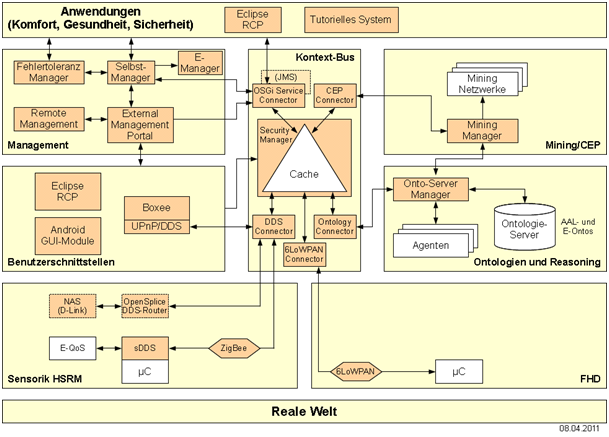
\includegraphics[scale=0.8]{images/wiedas_plattform}
\caption{WieDAS-Plattform}
\label{abb_wiedas_plattform}
\end{figure}

Auf die WieDAS-Plattform (Abbildung \ref{abb_wiedas_plattform}) wird von Benutzern über Anwendungen zugegriffen.
Diese Anwendungen liefern Mess- und Zustandsinformationen von Sensoren und steuern Aktoren.
Für zusätzliche Hilfestellung beim Bedienen der Anwendungen steht in der Architektur ein
tutorielles System bereit.
Die Plattform kann über Fernwartung oder andere verbundene Management-Module verwaltet werden.
Weiterhin stellt die Plattform Verwaltungseinheiten für den Betrieb bereit, z.B. das Sicherheits-Management.
Es werden fehlertolerante Dienste angeboten, welche den implementierten Diensten überlagert sind und die
Fehlertoleranz durch Redundanz erreicht.

Der Kern der Plattform ist der Kontext-Bus.
Er besteht aus verschiedenen Adaptermodulen (im weiteren Connectoren).
Die zentrale Einheit des Busses (im weiteren Cache) lagert die vorliegenden Daten und bietet sie
den angeschlossenen Modulen (Management- und Connectormodule) über eine Schnittstelle an.
Der Kontext-Bus spielt die zentrale Rolle dabei, Geräte die in der heterogenen Einsatzumgebung vorkommen, zu
homogenisieren.

Zur realen Welt liegt die Schnittstelle der Sensorik.
Hier befinden sich Sensoren, welche Messwerte \cite[Plattform]{wiedas} in den WieDAS-Datenraum befüllen oder
Schalt- und Regelungshardware, die Befehle im WieDAS-Datenraum bekannt geben.
In der realen Welt befinden sich weiter Aktoren, welche aus dem System heraus angesprochen werden können
und wiederum Aktionen in WieDAS selbst ausführen können.
Durch die Homogenisierung im Kontext-Bus soll z.B. der Sensor eines bestimmten Herstellers in der
Lage sein, einen Aktor eines anderen Herstellers zu steuern oder mit Informationen zu befüllen.

Die Plattform enthält weitere Module für z.B. Mining und Reasoning, die für die Entwicklung
der Software keine Relevanz besitzen.

\subsection{Datenmodell}
\label{gru_wiedas_daten}

% TODO KROEGER (klarer trennen: geräte, ifaces, datenraum), datenraum entspricht variablenmenge, insgesamt wenig exakt und formal
Das WieDAS-Datenmodell entspringt aus einer IDL-Datei \cite{wiedas_idl}.
Eine IDL-Datei ist ähnlich aufgebaut wie eine Schnittstellenbeschreibung in der Programmiersprache C.
In diesem Modell sind zum derzeitigen Zeitpunkt mehrere Sensoren, Kommandos und Funktionen hinterlegt.
Sie sind speicherschonend aufgebaut und besitzen wenig Informationen.
Die IDL-Datei ist mit Kommentaren versehen, wodurch man in der Lage ist, die verschiedenen Typen und Attribute
korrekt zu interpretieren.
Es existieren wenige primitive Datentypen, darunter z.B. eine ID, Schaltzustände oder Aufzählungen.
Weiterhin werden gewöhnliche Aufgaben, wie das Erfassen einer Temperatur, das Schalten, oder ähnliches
in Funktionalitäten zusammengefasst.
Die Geräte besitzen kaum spezifische Daten, dafür jedoch aussagekräftige kleinere Daten.
Das liegt zum Einen daran, dass WieDAS versucht, Geräte verschiedener Hersteller einzubinden und zum
anderen daran, dass sich der Speicherverbrauch der Geräteinformationen im AAL-Cache deutlich steigt,
wenn einfache Gerätefunktionen mit mehreren Daten abgebildet werden.
Geräte besitzen stets eine 16-Bit ID zur eindeutigen Identifizierung des Geräts im Datenraum.
Einzelne speziellere Geräte besitzen eine eigene Struktur, welche wiederum genauso aufgebaut sein
kann, wie eine Funktionalität oder andere Geräte.
Manche Strukturen sind auskommentiert oder besitzen Kommentare, die besagen, dass die Strukturen
nur vorläufig sind.
Zum Beispiel ist die Struktur eines Wasserstandsmelders identisch mit der Datenstruktur einer
normalen Lampe, da sie beide nur Informationen bezüglich des Einschaltzustands haben (An oder Aus).
Sind diese Geräte komplexer, wie z.B. eine dimmbare Lampe oder eine einstellbare Steckdose, so werden
weitere Parameter dieser Geräte mit vorher spezifizierten primitiven Datentypen oder den
Zahlentypen aus der IDL-Spezifikation erweitert.

\begin{absolutelynopagebreak}
\lstset{language=IDL}
\begin{lstlisting}[frame=single,caption={Gerätebeschreibung eines dimmbaren Lichts in WieDAS},label={devcode}]
typedef unsigned short deviceID_t;
enum OnOff { off, on };
typedef OnOff OnOffState_t;
struct DimmableLight_dt {
	deviceID_t id;
	octet LightIntensityState;
	OnOffState_t state;
};
\end{lstlisting}
Quellcode \ref{devcode} zeigt ein typisches Gerät.
Es besteht aus einer ID (Zeile 5) und einen oder mehrere für die Funktion relevanten Datentyp(en) (Zeile 6 und 7).
Falls Typen verwendet werden, die nicht in IDL spezifiziert sind, müssen diese vorher benannt werden (Zeile 1, 2 und 3).

\end{absolutelynopagebreak}

\subsection{AAL-Cache}
\label{gru_aalcache}

AAL-Cache ist die zentrale Softwarekomponente des Kontext-Busses des WieDAS-Projekts.
Die Kernaufgabe des AAL-Cache ist die Erfassung und Speicherung von Gerätedaten aus dem Umfeld.
Der Cache wird auf Multiprozessorsystemen eingesetzt \cite{aalcache}.
Darunter zählen auch Geräte im Netzwerk wie DSL-Router oder NAS-Systeme.
Er ist in C++ implementiert und bietet C- und Java-Schnittstellen zur Interaktion mit dem Cache.

Für jeden Cache-Eintrag speichert der AAL-Cache URIs mit dazugehörigen binären anwendungsspezifischen
Daten.
Die URIs dienen als Schlüssel und Identifikator für Cache-Einträge.
Aus Performancegründen sind die Einträge Maschinenworte, sogenannte Tags.
Die Tags werden mit einer Hashing-Funktion erstellt, die eine breite Verteilung besitzt
und gut auf verschiedenen Schlüsseln arbeiten soll \cite{aalc_hash}.
Registriert der Client ein URI, so erstellt der AAL-Cache eine neue Zuordnung, und ein Tag
für diese Zuordnung wird zurückgeliefert.
Damit die Liste der registrierten Tags und der verwendete Speicher nicht zu groß werden
besitzt der Kern eine feste Anzahl von ``Inodes''.
Inodes sind die zentralen Datenblöcke des AAL-Cache.
Sollte ein Tag nicht direkt verfügbar sein, so kann mittels einer Konstanten im Quellcode
die Anzahl der Wiederholungen eingestellt werden, die benutzt werden, um einen freien Tag zu ermitteln
\cite{aalcache}.
Wird ein Tag durch das verwendete Least-Recently-Used-Verfahren aus dem Kern verdränkt, so wird
der Connector darüber informiert.
Dieser muss dann die Verwendung des Tags bzw. die mit ihm verbundenen Daten abbrechen.

Weiterhin speichert der Cache einige Metadaten für jedes Datum, darunter z.B. die Identifikation
des Schreibers, 2 Zeitstempel, sowie den Energiebedarf zur Erhebung des Werts \cite{aalcache}.
Die Zeitstempel werden bei Lese- und Schreibzugriffen aktualisiert.
Zum Zwecke der Lesbarkeit des Datums wird weiterhin ein Datentyp-Hint hinterlegt.

Die Abbildung \ref{abb_aalcache} zeigt, welche Komponenten in der AAL-Cache Architektur verwendet werden.
\begin{figure}[h]
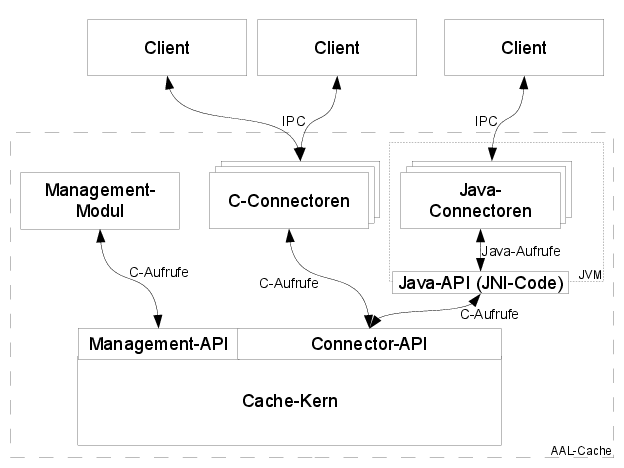
\includegraphics[scale=0.7]{images/aalcache}
\caption{Architektur des AAL-Cache}
\label{abb_aalcache}
\end{figure}

Damit die herstellerspezifischen Geräte und Protokolle vom AAL-Cache verarbeitet werden können, schreiben
die Softwareentwickler, die mit dem Cache arbeiten, Adaptermodule (im weiteren Connectoren).
Die Connectoren sind die Verbindung zur realen Welt.
Sie interagieren mit den Produkten für Sensorik und Steuerungseinheiten.
Es können auch Anwendungen für Benutzer oder weitere Module geschrieben werden,
die die Daten aus dem Cache verarbeiten wollen.
Connectoren werden stets im Kontext des AAL-Cache Prozesses ausgeführt \cite{aalcache}.
Der Cache läuft ständig und kann mittels der geschriebenen Connectoren, welche
für die Hersteller spezifische Codestücke enthalten, Daten aus der Umgebung erfassen bzw. in diese verbreiten.
Dadurch, dass der Prozess dauerhaft läuft, werden die Connectoren als Arbeiter realisiert und laufen in
separaten Threads.
Connectoren sind somit eng mit dem AAL-Cache gekoppelt.
Dadurch ist die Kommunikation zwischen den Clients, also den Nutzern der API, und dem Kern gewährleistet.
Nachrichten werden entweder über eine registrierte Callback-Funktion oder aber über das explizite
Anfordern/Einpflegen von Daten übermittelt.
Die Connectoren können wiederum selbst Threads benutzen.
Connectoren werden entweder zum Startzeitpunkt geladen oder können während der Laufzeit geladen werden.
Der AAL-Cache stellt für diese eine Schnittstelle bereit, welche beim Starten der Connectoren
verwendet wird, um sich beim AAL-Cache zu registrieren.
Das Programm bedient sich dabei der Möglichkeit, unter Linux dynamische Bibliotheken zu laden.
Wie die Abbildung \ref{abb_aalcache} zeigt, existieren derzeit die Möglichkeiten, eine Implementierung
von Connectoren in
\begin{enumerate}
\item C
\item Java
\end{enumerate}
vorzunehmen.

Die Java-Connectoren bedienen sich dabei einer Java VM, die über JNI-Code auf der C-Schnittstelle aufsetzt.
Der Cache selbst ist in C++ verfasst, bietet jedoch eine C-Schnittstelle, so dass auch Implementierungen von
Connectoren in purem C ermöglicht werden, um z.B. den Speicherverbrauch geringer zu halten.
Im aktuellen Code-Repository \cite{aalcache_code} befinden sich bereits Connectoren für z.B. OSGi,
Ontology-Homeautomation, DDS und sDDS.

Möchte der Connector über Ereignisse zu einem URI informiert werden, so muss er
eine Registrierung am Kern vornehmen.
Dazu werden die gewünschten Tags an eine Registrierungsfunktion übergeben, welche
dann wiederum ein Subscription-Set liefert.
Dieses kann dann auch wieder zum Auflösen der Registrierungen verwendet werden.
Bei der Registrierung wird Tags und die Anzahl der übergebenen Tags mitgeliefert.
Wird ein registriertes Callback ausgeführt, so kann es vorkommen, dass dies in einem anderen
Thread passiert.

Um auf die Daten im Cache zuzugreifen, bietet die Schnittstelle die Funktion \emph{getCopy}
und \emph{getLock}.
Die erste Funktion liefert eine Kopie der Metadaten und des gespeicherten Datums.
Sie können verändert werden und zurück in den Cache geschrieben werden.
Die 2. Funktion gibt einen Zeiger auf das interne Datum zurück.
Dieser kann nicht für Schreibzugriffe verwendet werden und muss mittels \emph{unlock}
wieder für Schreibzugriffe freigegeben werden.

\vfill
\pagebreak

%TODO KROEGER (schnittstellenbeschreibung der .h?)
Der Cache selbst kann zur Laufzeit mittels der Management-Schnittstelle konfiguriert werden.
Funktionen, die die dynamische Verwaltung erlauben, umfassen:
\begin{enumerate}
\item Anlegen von Speicherpools, falls die vorkonfigurierte Anzahl nicht ausreichend sein sollte
\item Laden von Connectoren, durch Angabe von Dateinamen und der benötigten Funktionen
\item Statusabfragen (z.B. Liste aller Connectoren, Anzahl belegter/gesamter Inodes, Zugriffszähler)
\item Zurücksetzen der Zugriffszähler
\end{enumerate}
Da manche Konfigurationen nicht zur Laufzeit vorgenommen werden können (Anzahl der Inodes, Threads,
Callback-Warteschlangenlänge), werden diese statisch konfiguriert.
Der Cache wird mit XML-Daten konfiguriert, worin auch die dynamisch konfigurierbaren Einstellungen
initial vorgenommen werden.

\section{XML-RPC}
\label{gru_xmlrpc}

XML-RPC ist ein entfernter Prozeduraufruf unter der Benutzung von XML.
Es bedient sich, wie der Name verrät, an der weit verbreiteten und anerkannten Interprozesskommunikationstechnik
RPC (Remote Procedure Call).
Wie der Begriff verrät, findet man RPC in verteilten Systemen, wo der Aufrufer eine gewisse
Aufgabe ausgeführt haben möchte und einen Aufruf absetzt.
Der Aufrufer oder Sender wird Client und der Empfänger, welcher die Aufgabe ausführt, Server genannt.

Für den Programmierer ist der Aufruf selbst nicht von einem lokal ausgeführten Aufruf zu unterscheiden.
Der Programmierer sorgt lediglich für den Verbindungsaufbau zum Server.
Die Transportmechanismen sind dabei für den Programmierer nicht sichtbar und befinden sich in den jeweiligen
Implementierungen.
Für den Transport zwischen den Teilnehmern werden Nachrichten genutzt, dadurch muss die Implementierung
des Protokolls eine Kodierung (sogenanntes Marshalling) vornehmen.

Für dieses Marshalling bzw. den Transport selbst kann XML verwendet werden.
XML-RPC jedoch ist ein eigenständiges Protokoll, welches ein gewisses Nachrichtenformat erwartet und vordefinierte
Datentypen besitzt.
Anwendungsspezifische Datentypen können mittels der primitiven Datentypen, die von XML-RPC bereitgestellt werden,
zusammengebaut werden.
XML-RPC ist durch das vordefinierte Nachrichtenformat und den Verlust der anwendungsspezifischen Datentypen
und Kompaktifizierung etwas größer als reines XML \cite{xmlrpc_so}.

XML-RPC bietet gegenüber RPC über XML z.B. Vorteile durch:
\begin{enumerate}
\item Einfache Datentypen (String, Integer, usw.).
\item Standardisiertes Datumformat
\item Häufige Integration der Transportschicht in den Bibliotheken
\end{enumerate}
\lstset{language=XML}
\begin{lstlisting}[frame=single,caption={Aufbau einer XML-RPC-Nachricht},label={aufbau_xmlrpc}]
POST /RPC2 HTTP/1.0
User-Agent: Some/Browser
Host: somewhere.com
Content-Type: text/xml
Content-length: 181

<?xml version="1.0" encoding="ISO-8859-1"?>
<methodCall>
	<methodName>sample.sum</methodName>
	<params>
		<param>
			<value><int>17</int></value>
		</param>
		<param>
			<value><int>13</int></value>
		</param>
	</params>
</methodCall>
\end{lstlisting}
Der Aufbau einer XML-RPC-Nachricht wird in Quellcode \ref{aufbau_xmlrpc} gezeigt.
Dieser entspringt der Spezifizierung des XML-RPC \cite{xmlrpc}.

Während bei einer Verwendung von XML für RPC der Transportmechanismus keine Rolle spielen würde, findet
der Aufruf eines XML-RPC über HTTP statt, wie es in den Zeilen 1 bis 5 in Quellcode \ref{aufbau_xmlrpc} zu sehen ist.
Dies bietet einen Vorteil beim Feststellen von Fehlern oder der Kommunikation, welcher aber gleichzeitig
ein Nachteil während des Betriebs ist, da die Kommunikation zwischen den beteiligten Komponenten
eingesehen werden kann.
Die Pfadangabe im POST-Request in der ersten Zeile des Requests ist nicht näher spezifiziert.
Er kann allerdings dafür genutzt werden in einem Webserver, der mehrere Requests bearbeitet, dem entsprechenden
Verarbeitungsprogramm zukommen zu lassen.
Der übertragene Inhalt ist ein XML Dokument (Zeile 4).
Die Wurzel der XML-Datenstruktur, die beim Aufruf verwendet wird, ist \emph{methodCall} (Zeile 8).
Darin befinden sich Informationen wie der Name der Methode (Zeile 9) und den benötigten Parametern (Zeile 12 und 15).
Die Parameter sind nicht benannt und werden durch die Spezifizierung der Methode festgelegt.
Es ist möglich, durch das Verwenden des Methodennames \emph{system.multicall} mehrere Requests
in einer Nachricht zu kapseln.

Eine Antwort des XML-RPC Servers verwendet statt des \emph{methodCall}-Elements das \emph{methodResponse}-Element.
Wurde der Request verarbeitet, so kann der Server die entsprechende Antwort zurückliefern.
Dabei wird allerdings nur ein einziger Wert benutzt.
Dies kann allerdings ein Array sein.
Bei der Verwendung von \emph{system.multicall} wird ein Array mit je einer Name-Wert-Assoziation
für einen Methodenaufruf zurückgegeben.

Wird ein Fehler bei der Verarbeitung festgestellt, so liefert der Server im \emph{methodResponse}-Element
ein \emph{fault}-Element zurück \cite{xmlrpc}.
Darin befindet sich ein Mapping mit einem Code und einer Zeichenkette, die den Fehler identifiziert.
Die Fehlercodes sind nicht spezifiziert und können von der Implementierung frei verwendet werden.

\section{HomeMatic-Hausautomation}
\label{gru_hm_ha}

HomeMatic ist ein Protokoll der Firma eQ-3 und wird in der Haus- und Gebäudeautomation
verwendet.
HomeMatic-Hausautomation bietet verschiedene Geräte für die Hausinstallation und wirbt damit,
einfach bedienbar, zuverlässig, sicher und erweiterbar zu sein \cite{homematic_eq3}.

Die Produktserie wird in mehrere Kategorien aufgeteilt.
\begin{enumerate}
\item{Zentralen und Gateways}
\item{Sender und Controller}
\item{Sensoren}
\item{Aktoren}
\end{enumerate}

Das Funk-Kommunikationsprotokoll, welches für die Geräte eingesetzt wird, heißt BidCoS®.
Das Protokoll ist bidirektional und bestätigt empfangene Daten.
Es bietet weiterhin Sicherheitsmerkmale, z.B. die verschlüsselte Kommunikation.
Es wurde speziell für die drahtlose Ansteuerung der Geräte entwickelt \cite{homematic_eq3_faq} (BidCoS®-RF),
wird jedoch auch für die Kommunikation über Kabelverbindungen genutzt (BidCoS®-Wired).

Um eine komfortable Steuerung und Verwaltung der im Haus befindlichen Geräte durchzuführen,
bietet HomeMatic Stationen an, die als Zentrale oder Gateway dienen.
Die Zentrale der HomeMatic-Umgebung ist die HomeMatic-CCU.

\subsection{HomeMatic-CCU Zentrale}
\label{gru_hm_ccu}

Die Geräte in der HomeMatic-Umgebung können über Funk oder Kabel mit der Zentrale verbunden
werden.
Um die Zentrale nicht zwangsläufig in der nähe des PC aufzustellen, der sie konfiguriert,
bietet HomeMatic weitere Adapter und Gateways an, um so z.B. Konfiguration mit USB-Sticks vorzunehmen.

Die HomeMatic-CCU bietet Möglichkeiten, mit der Sensorik auf verschiedene Art und Weise zu
interagieren \cite[Seite 6]{homematic_ccu}.
Die Anwendung, die dafür bereitgestellt wird, heißt HomeMatic-WebUI \cite{homematic_webui_manual}
und kann folgende Aufgaben bewältigen:
\begin{enumerate}
\item Konfiguration und Bedienung der Geräte
\item Abfrage von Statusinformationen
\item Herstellen von Verknüpfungen unter den Geräten
\item Komplexere Funktionen über Zentralprogramme realisieren
\end{enumerate}

Es existieren derzeit 2 Verbindungsmöglichkeiten zur Steuereinheit \cite[Seite 10]{homematic_ccu}:
\begin{enumerate}
\item USB-Steckverbindung
\item Ethernet-Steckverbindung
\end{enumerate}

Je nach Lage des Systems an dem die Steuereinheit angeschlossen werden soll und wie sie konfiguriert
werden muss, kann eine Verbindung bevorzugt werden.
Dabei ist zu beachten, dass die USB-Verbindung nur unter Windows Betriebssystemen
verwendet werden kann.
Dort wird dann eine Netzwerkkarte emuliert.
HomeMatic bietet mit \emph{NetFinder} eine eigene Software an, um eine oder mehrere
HomeMatic-CCU im Netzwerk zu erkennen.

Durch das Verwenden von HTTP bei WebUI ist man auch in der Lage, die Zentrale
über das Internet, z.B. durch die Verwendung von Smartphones zu konfigurieren.
Dazu müssen lediglich die Aufrufe aus dem Internet an die Zentrale weitergeleitet werden
(Router-Portforwarding).

Die HomeMatic-CCU benötigt nur für das Stellen der Uhrzeit Zugriff auf das Internet.
Je nach Netzwerkkonfiguration im Hause können die Netzwerkkonfiguration sowie Zeitserver
für die Zentrale manuell konfiguriert werden.
Die Uhrzeit kann aber auch vollständig manuell eingestellt werden, um die Anlage
funktionsfähig zu machen.

HomeMatic bietet zur Ansteuerung von Aktoren moderne Funk-Fernbedienungen mit verschiedenen
Anzahlen von Tastern, sowie Möglichkeiten, Taster in Gebäude-Elektroinstallationen unterputz anzubringen.
Um automatisch Werte aus der Hausinstallation zu erfassen, gibt es verschiedene Sensoren für z.B.
Wetter, Rauch, Bewegung und elektrische Impulserkennung.
Als Aktoren dienen Dimmer, Unterputzeinsätze für vorhandene Installationen, einfache Ausgangsmodule und
komplexe Steuerungsmodule für z.B. Heizung oder Türgriffe.
Um komplexere Steuerungen zu realisieren, bietet HomeMatic die Möglichkeit, Scripts in der Zentrale
zu hinterlegen \cite{hmscript1}.

Um eine Verbindung zwischen den Geräten und der Zentrale herzustellen, müssen die Geräte zunächst
angemeldet werden.
Voraussetzung dafür ist das korrekte Setzen der Uhrzeit (s.o.) in der Zentrale und das eventuelle
Aktualisieren der installierten Firmware.
Ist die Zeit gesetzt (es blinken keine Status-LED am Gerät) ist die Zentrale bereit, Anmeldungen
durchzuführen.
Eine Anmeldung wird prinzipiell durch Klicken auf den ``Teach-In Devices''
in der WebUI an der Zentrale eingeleitet.
Die Sequenz am Gerät ist spezifisch und ist in den Bedienungsanleitungen hinterlegt.

Für die verfügbaren Geräteverbindungen (Kabel, Funk, Intern) existieren Programmierschnittstellen.
Es können Verknüpfungen zwischen Geräten mittels der Browseranwendung im WebUI vorgenommen werden.
Dabei kann man sich mit Dropdown-Boxes die gewünschten Geräte und die entsprechenden Funktionen
ausgewählt und dann verknüpft werden.
Weiterhin kann man Programme oder Programmsammlungen aus dem Internet herunterladen und der CCU
übergeben, um komplexere Verknüpfungen nicht selbst herstellen zu müssen.

Als Alternative können Programme über die Verwendung der XML-RPC-Schnittstelle \cite[Seite 4]{homematic_xmlrpc}
realisiert werden.
Diese Programmierschnittstellen verwenden das im Abschnitt \ref{gru_xmlrpc} beschriebene XML-RPC-Protokoll.
Die Nutzung der Schnittstelle unterscheidet dabei zwischen dem Schnittstellenprozess und dem Logikprozess.

%\vfill
%\pagebreak

\begin{figure}[h!]
\includegraphics[scale=0.8]{images/ccu_logic_iface}
\caption{Schnittstellen- und Logikprozesse}
\label{abb_ccu_logic_iface}
\end{figure}
%TODO DANIEL (herr kröger hat hier [3] in der caption hintergeschrieben)
Die Abbildung \ref{abb_ccu_logic_iface} zeigt, wo sich die Prozesse befinden.
Ein Logikprozess kann mit mehreren Schnittstellenprozessen kommunizieren \cite[Seite 3]{homematic_xmlrpc}.
Dazu meldet die Anwendung den Logik- bei dem Schnittstellenprozess an, welcher sich dann wiederum diesen
Prozess mit einer ID merkt.
Der Schnittstellenprozess wird von der HomeMatic-CCU angeboten und dient der expliziten Steuerung
bzw. dem Anfordern von Informationen.
Die Schnittstelle bietet manche Methoden immer an und manche nur optional \cite[Seite 14]{homematic_xmlrpc}.
Der Logikprozess ist auf der Seite der Anwendung (bzw. des Programms) und ist der Prozess, welcher die
Aufrufe tätigt oder auch vom Schnittstellenprozess über bestimmte Ereignisse oder neue Geräte
benachrichtigt wird.
Er muss bestimmte XML-RPC-Methoden \cite[Seite 22]{homematic_xmlrpc} bereitstellen.

Durch bestimmtes Verhalten des Logikprozesses kann die Schnittstelle einen Abgleich über vorhandene
Geräte durchführen.
Die Logik-Schnittstelle wird bei der An- und Abmeldung von neuen Geräten mit dem Aufruf von \emph{newDevices}
bzw. \emph{deleteDevices} \cite{homematic_xmlrpc} darüber informiert.
Es überträgt dabei die Gerätebeschreibungen für die hinzugefügten Geräte.
Der Abgleich kann durchgeführt werden, wenn sich die Logikschnittstelle die Gerätebeschreibungen
merkt \cite[Seite 22]{homematic_xmlrpc} und entsprechend der Aufrufe modifiziert.
Dazu müssen nur die Schlüssel \emph{ADDRESS} und \emph{VERSION} gespeichert werden und bei einem
Aufruf von \emph{listDevices} zurückgeliefert werden.
Der Logikprozess sieht dabei Beschreibungen für alle \emph{logischen} Geräte \cite[Seite 3]{homematic_xmlrpc}.
Das heißt, dass  bei der Übergabe der Adresse bei einem Ereignis (\emph{event}-Funktion der
Logikschnittstelle) auch Kanaladressen übergeben werden.

Die CCU stellt für jede Verbindungsart der Geräte einen Schnittstellenprozess bereit.
Diese Prozesse sind XML-RPC-Server und laufen unter jeweils einem anderen Port.
\begin{enumerate}
\item Port 2000 für drahtgebundene Komponenten
\item Port 2001 für Funk-Komponenten
\item Port 2002 für interne Komponenten
\end{enumerate}
Die XML-RPC-Server stehen unter der vergebenen IP-Adresse (s.o.) und dem entsprechenden Port
zur Verfügung und werden über HTTP angesprochen.
Der Logikprozess muss, falls er benutzt werden soll, an einer IP-Adresse und auf einem Port auf
eingehende Verbindungen warten, die für den Schnittstellenprozess erreichbar ist.
Um eine Zugriffsbeschränkung für die XML-RPC-Schnittstelle festzulegen, kann in der WebUI-Oberfläche
der Zugriff entweder komplett verboten, komplett erlaubt oder IP-basiert festgelegt werden \cite[Seite 92]{homematic_webui_manual}.

\subsection{HomeMatic-Gerätemodell}
\label{gru_hm_obj}

Die Geräte werden aus einer Menge von Kanälen modelliert \cite[Seite 13]{hmscript2}, in welchen
die eigentliche Funktionalität steckt \cite[Seite 16]{hmscript2}.
Diese Funktionalität wird in Datenpunkten abgebildet.
Ein Gerät wird über eine Adresse identifiziert.
Jedes Gerät besitzt eine verschiedene Anzahl von Kanälen unterschiedlichen Typs mit
verschiedenen Datenpunkten.
Die Datenpunkte werden dann entweder ausgelesen, um Zustände von Geräten zu erfahren, oder gesetzt,
um Funktionalitäten zu erfüllen.

Der Schnittstellenprozess der CCU behandelt nur logische Geräte \cite{homematic_xmlrpc}.
Somit werden auch Funktionen der Geräte als eigenständiges Gerät bezeichnet und
erhalten eine eigenständige Adresse.
Ein Multifunktionsgerät könnte folgendermaßen adressiert werden:
\begin{itemize}
\item ABC123 Gerät selbst
\item ABC123:1 Schaltausgang 1
\item ABC123:3 Schalteingang 3
\end{itemize}

Die Datenpunkte sind typisiert, haben bestimmte Eigenschaften und Metadaten \cite[Seite 21]{hmscript2}.
Die Eigenschaften und Metadaten eines Datenpunkts sind der aktuelle typisierte Wert, den letzten Wert
(z.B. sinnvoll für dimmbare Aktoren), die Operationen, die auf dem Datenpunkt ausgeführt werden können,
und den Zeitstempel der letzten Aktualisierung.

Die Kanäle und die dazugehörigen Datenpunkte der zur Zeit verfügbaren Geräte sind
spezifiziert \cite{hmscript4}.
Die Tabelle \ref{tab_hm_chan} und Tabelle \ref{tab_hm_dp} zeigen Ausschnitte aus dem Modell für ein
HomeMatic-Funk-Wandthermostat \cite[Seite 12]{hmscript4}.

\begin{table}[h]
\begin{tabular}{|l|l|l|}
\hline
Kanaltyp & Kanalnummer \\
\hline
WEATHER & 1 \\
\hline
CLIMATECONTROL\_REGULATOR & 2 \\
\hline
\end{tabular}
\caption{Kanaltypen eines HomeMatic-Wandthermostats}
\label{tab_hm_chan}
\end{table}

\begin{table}[h]
\begin{tabular}{|l|l|l|l|}
\hline
Kanal & Name & Typ & Zugriff \\
\hline
1 & TEMPERATURE & float & lesend und über Ereignisse \\
\hline
2 & SETPOINT & boolean & lesend, schreibend und über Ereignisse \\
\hline
\end{tabular}
\caption{Datenpunkte eines HomeMatic-Wandthermostats}
\label{tab_hm_dp}
\end{table}

Tabelle \ref{tab_hm_chan} zeigt, dass das Thermostat 2 Kanäle besitzt.
Ein Kanal existiert für die Zustandsinformationen bezüglich der Wetterdaten, ein anderer
für das Interagieren mit der Regulierung.
Die Datenpunkte in Tabelle \ref{tab_hm_dp} sind beide direkt auszulesen oder können
Ereignisse auslösen (z.B. wenn sich die Raumtemperatur ändert oder die Solltemperatur
gesetzt wird).

Nicht aufgezeigt sind in dieser Tabelle weiterführende Attribute der Datenpunkte, welche
den Wert genauer beschreiben \cite[Seite 3]{hmscript4}.

\begin{itemize}
\item Minimalwert
\item Maximalwert
\item Standardwert
\item Einheit
\item Spezielle Werte
\end{itemize}

Diese Wertebeschreibung ist nur dort vorhanden, wo der Datentyp numerisch ist.
Spezielle Werte treten auf, um bestimmte Zustände zu beschreiben.
Zum Beispiel gibt es für den Datenpunkt \emph{SETPOINT} in Tabelle \ref{tab_hm_dp}
die speziellen Werte \emph{VENT\_CLOSED} und \emph{VENT\_OPEN}, um den Zustand des angeschlossenen
bzw. gekoppelten Ventils zu beschreiben.
Diese Werte sind speziell zu interpretieren und liegen außerhalb des Wertebereichs
(hier 0 und 100).

Datenpunkte werden mit ihrem Namen und dem dazugehörigen Wert im XML-RPC-Request als Parametersets
zusammengefasst.
Parametersets sind wiederum noch einmal nach Typ kategorisiert.
\begin{enumerate}
\item MASTER dient der Konfiguration eines Geräts
\item LINK offeriert ein Parameterset zur Beschreibung einer Verknüpfung zwischen Kanälen
\item VALUES ist das Set, welches die Messwerte, Statusinformationen und Schaltzustände beschreibt
\end{enumerate}
Tabelle \ref{tab_hm_dp} zeigt den Ausschnitt aus einem \emph{VALUES} Parameterset.
Parametersets haben Beschreibungen, die ebenfalls mit Funktionen vom Schnittstellenprozess
angefordert werden können.

Eine Dokumentation darüber, wie die Datenpunkte zu interpretieren sind, liegt leider nicht vor.
In der Dokumentation wird lediglich der Wertebereich bzw. der Typ des Datenpunkts gegeben.
Anhand dieser Informationen kann man Datenpunkte gekoppelt mit dem Namen des Datenpunkts
kann eine Annahme über die Funktion des Datenpunkts getroffen werden.
In der Analyse muss herausgefunden werden, wie hier eine geeignete Abbildung gefunden werden kann.
